%!TEX TS-program = xelatex
%!TEX options = -aux-directory=Debug -shell-escape -file-line-error -interaction=nonstopmode -halt-on-error -synctex=1 "%DOC%"
\documentclass{article}
\input{LaTeX-Submodule/template.tex}

% Additional packages & macros
\DeclareMathOperator{\sgn}{sgn}
\usepackage{makecell}

% Header and footer
\newcommand{\unitName}{Telecommunications and RF}
\newcommand{\unitTime}{Semester 2, 2023}
\newcommand{\unitCoordinator}{Dr Jacob Coetzee}
\newcommand{\documentAuthors}{Tarang Janawalkar}

\fancyhead[L]{\unitName}
\fancyhead[R]{\leftmark}
\fancyfoot[C]{\thepage}

% Copyright
\usepackage[
    type={CC},
    modifier={by-nc-sa},
    version={4.0},
    imagewidth={5em},
    hyphenation={raggedright}
]{doclicense}

\date{}

\begin{document}
%
\begin{titlepage}
    \vspace*{\fill}
    \begin{center}
        \LARGE{\textbf{\unitName}} \\[0.1in]
        \normalsize{\unitTime} \\[0.2in]
        \normalsize\textit{\unitCoordinator} \\[0.2in]
        \documentAuthors
    \end{center}
    \vspace*{\fill}
    \doclicenseThis
    \thispagestyle{empty}
\end{titlepage}
\newpage
%
\tableofcontents
\newpage
%
\section{Telecommunications Systems}
Telecommunication is the transmission of information over a distance through some technology.

Telecommunications systems are designed to transmit information with
as little \textbf{deterioration} as possible while satisfying design constraints, such as
allowable transmittable energy and signal bandwidth.

Signal deterioration commonly measures:
\begin{itemize}
    \item For Analog Systems: \textbf{Signal-to-Noise Ratio} (SNR) at the receiver output --- the ratio of the signal power to the noise power
    \item For Digital Systems: \textbf{Bit Error Rate} (BER) at the receiver output --- the ratio of the number of bits received in error to the total number of bits transmitted
\end{itemize}
\subsection{Analog and Digital Signals}
A system is either \textbf{analog} or \textbf{digital} based on the possible amplitudes of waveforms it can handle.
\begin{itemize}
    \item \textbf{Analog Information Sources} produce values defined on a continuum:
          \begin{itemize}
              \item Human voice and other sounds
          \end{itemize}
    \item \textbf{Digital Information Sources} produce a finite set of possible symbols:
          \begin{itemize}
              \item Computer data
              \item MP3 encoder output
          \end{itemize}
\end{itemize}
\subsection{Communications System}
A communications system can be summarised by the following block diagram:
\begin{figure}[H]
    \centering
    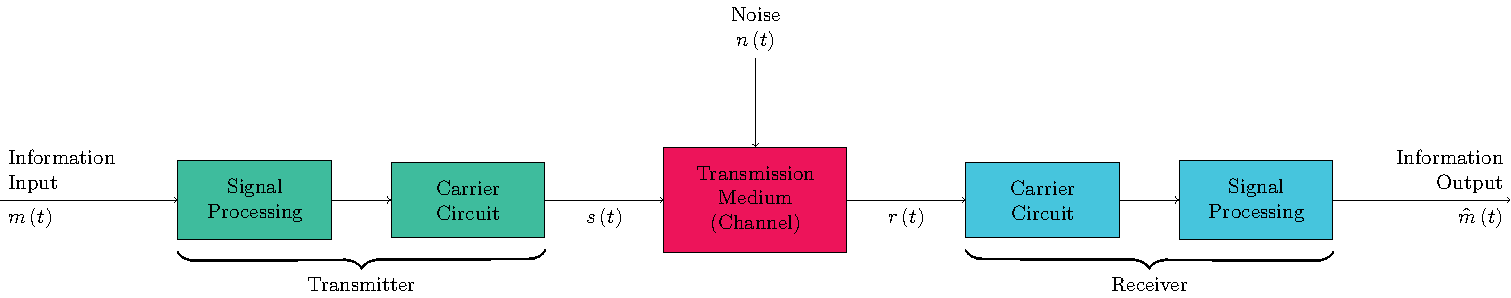
\includegraphics[width=\linewidth]{figures/communications_system.pdf}
    % \caption{} % \label{}
\end{figure}
where
\begin{itemize}
    \item \(m\left( t \right)\) is the information message signal (prior to conditioning for transmission)
    \item \(s\left( t \right)\) is the conditioned signal for transmission
    \item \(n\left( t \right)\) contains channel noise and interference
    \item \(r\left( t \right)\) is the received signal
    \item \(\hat{m}\left( t \right)\) is the reconstructed received message signal (where \(\hat{m}\left( t \right)\) usually approximates \(m\left( t \right)\))
\end{itemize}
\subsubsection{Transmitter}
The transmitter carries out \textbf{signal conditioning} by transforming the signal to a more appropriate form before transmission through the channel.
Some examples of signal conditioning techniques are prodived below.
\begin{itemize}
    \item \textbf{Low Pass Filtering} (LPF) restricts signal bandwidth to avoid wasting signal power on frequencies that are not transmitted by the channel and to avoid interference with other signals
    \item \textbf{Analog to Digital Conversion} (ADC) produces a digital word which represents a sample of the analog message waveform
    \item \textbf{Carrier Modulation} transfers the signal to a frequency band that is suitable for transmission through the channel
\end{itemize}
\subsubsection{Channel}
A communication channel refers to the physical medium that carries the signal from the transmitter to the receiver.
There are two types of channels:
\begin{itemize}
    \item \textbf{Wired}: twisted pair copper telephone lines, waveguides, coaxial cables, fibre-optic cables
    \item \textbf{Wireless}: air, vacuums, sea water, optical fibres
\end{itemize}
General principles of communications always apply regardless of the type of channel. However, certain
conditioning methods are better suited to certain channels.

Channels often \textbf{attenuate} signals (reduce their amplitude or strength) through
\begin{itemize}
    \item random noise
    \item interference from other sources
\end{itemize}
and therefore it is a key consideration in the design of a communications system.
\subsubsection{Receiver}
The receiver acts as the inverse of a transmitter. The receiver:
\begin{enumerate}
    \item \textbf{Demodulates} the received signal by stripping the carrier from the received signal \(r\left( t \right)\).
    \item \textbf{Filters} out noise and interference from the demodulated signal.
    \item \textbf{Reconstructs} an estimate of the original message signal \(\hat{m}\left( t \right)\).
\end{enumerate}
Due to the finite nature of the SNR, the estimated output of an analog signal can never be exactly
equal to the original signal\footnote{A perfect reconstruction requires an infinite SNR which is impractical.}.
However, it is often possible to reconstruct a digital signal exactly
using error detection and correction techniques at the receiver.
\subsubsection{Information Sources}
As discussed before, an information source can be classified as either \textbf{analog} or \textbf{digital}.
Analog signals can be modulated or transmitted directly, or
converted to digital data and transmitted using digital modulation techniques.

An analogue signal to be transmitted is called the \textbf{message signal} and is denoted \(m\left( t \right)\).
The spectral components of this signal lie within a finite bandwidth \(W\), such that \(M\left( f \right) = 0\) for \(\abs*{f} > W\),
where \(M\left( f \right)\) is the Fourier Transform of \(m\left( t \right)\). This signal's bandwidth is limited to prevent
interference with other signals.

Many kinds of message signals can be considered:
\begin{itemize}
    \item Audio
    \item Video
    \item Computer data
    \item Telemetry (measurements)
    \item Soundings (RADAR, SONAR)
    \item A mixure of the above (i.e., data over voice)
\end{itemize}
\subsection{Modulation}
The process of modulation produces a signal that is suitable for transmission through the channel
by transforming the message signal \(m\left( t \right)\) to a new signal \(s\left( t \right)\).

Modulation is often performed with respect to another signal, called the \textbf{carrier} signal \(c\left( t \right)\).
Here the message \textit{modulates} the carrier to produce the transmitted signal \(s\left( t \right)\).
\subsubsection{Benefits of Modulation}
\begin{itemize}
    \item Modulation shifts the spectral content of a message onto a suitable band.
          As the size of an antenna is related to the wavelength of a signal, higher carrier frequencies require smaller antennas.
    \item Modulation facilitates multiplexing, where multiple signals are transmitted over the same spectrum.
          This is because the frequency spectrum can be divided into non-overlapping frequency bands, each of which can carry a separate signal.
    \item Modulation provides some control over noise and interference by choosing a bandwidth that is smaller than the allocated channel bandwidth.
\end{itemize}
\subsubsection{Convolution and Modulation}
Consider two time domain signals \(m\left( t \right)\) and \(c\left( t \right)\) and their Fourier Transforms \(M\left( f \right)\) and \(C\left( f \right)\) respectively.

The \textbf{Convolution Property} demonstrates:
\begin{align*}
    m\left( t \right) \ast c\left( t \right) & = y\left( t \right) &  & \text{Convolution in Time Domain}         \\
    M\left( f \right) C\left( f \right)      & = Y\left( f \right) &  & \text{Multiplication in Frequency Domain}
\end{align*}
The \textbf{Modulation property} demonstrates:
\begin{align*}
    m\left( t \right) c\left( t \right)      & = y\left( t \right) &  & \text{Multiplication in Time Domain}   \\
    M\left( f \right) \ast C\left( f \right) & = Y\left( f \right) &  & \text{Convolution in Frequency Domain}
\end{align*}
\subsubsection{Carrier Signal}
The carrier signal \(c\left( t \right)\) is a sinusoidal signal of the form:
\begin{equation*}
    c\left( t \right) = A_c \cos{\left( 2 \pi f_c t + \phi \right)}
\end{equation*}
where \(A_c\) is the amplitude, \(f_c\) is the frequency and \(\phi\) is the phase of the carrier signal.
\subsubsection{Signal Properties}
The \textbf{energy} of a signal \(x\left( t \right)\) is defined as:
\begin{equation*}
    E_x = \int_{-\infty}^{\infty} \abs*{x\left( t \right)}^2 \odif{t}
\end{equation*}
The rate at which energy is transmitted is called the \textbf{power} of the signal, and is defined as:
\begin{equation*}
    P_x = \lim_{T \to \infty} \frac{1}{T} \int_{-T/2}^{T/2} \abs*{x\left( t \right)}^2 \odif{t}
\end{equation*}
where \(T\) is the time period over which the power is measured.
\subsection{Amplitude Modulation Schemes}
A message signal \(m\left( t \right)\) with bandwidth \(W\) can be amplitude modulated by
mixing (multiplying) the signal with a carrier signal \(c\left( t \right)\):
\begin{equation*}
    c\left( t \right) = A_c \cos{\left( 2 \pi f_c t \right)}
\end{equation*}
with amplitude \(A_c\) and carrier frequency \(f_c \gg W\).

This section will consider:
\begin{itemize}
    \item Double Side Band --- Suppressed Carrier (DSB-SC) modulation
    \item Double Side Band --- Full Carrier (DSB-FC) modulation, or simply conventional Amplitude Modulation (AM)
    \item Single Side Band (SSB) modulation
\end{itemize}
\subsubsection{Double Side Band --- Suppressed Carrier (DSB-SC)}
The transmitted signal is defined as:
\begin{equation*}
    s\left( t \right) = m\left( t \right) c\left( t \right) = A_c m\left( t \right) \cos{\left( 2 \pi f_c t \right)}.
\end{equation*}
In the frequency domain, the message signal is shifted to the carrier frequency at \(\pm f_c\) and the magnitude is halved.
\begin{equation*}
    S\left( f \right) = \frac{1}{2} A_c \left[ M\left( f - f_c \right) + M\left( f + f_c \right) \right]
\end{equation*}
Assuming no channel noise, the received signal can be represented as:
\begin{equation*}
    r\left( t \right) = s\left( t \right) = A_c m\left( t \right) \cos{\left( 2 \pi f_c t \right)}
\end{equation*}
This signal can be demodulated coherently by multiplying a sinusoidal signal of the same frequency as the carrier.
Suppose we generate the sinusoidal signal \(\cos{\left( 2 \pi f_c t + \phi \right)}\) where \(\phi\) is the phase of the sinusoid.
\begin{align*}
    y\left( t \right) & = r\left( t \right) \cos{\left( 2 \pi f_c t + \phi \right)}                                                                                                                                             \\
                      & = A_c m\left( t \right) \cos{\left( 2 \pi f_c t \right)} \cos{\left( 2 \pi f_c t + \phi \right)}                                                                                                        \\
                      & = \frac{1}{2} A_c m\left( t \right) \left[ \cos{\left( 4 \pi f_c t + \phi \right)} + \cos{\left( -\phi \right)} \right]                                                                                 \\
                      & = \underbrace{\frac{1}{2} A_c m\left( t \right) \cos{\left( \phi \right)}}_{\text{filter out}} + \underbrace{\frac{1}{2} A_c m\left( t \right) \cos{\left( 4 \pi f_c t + \phi \right)}}_{\text{reject}}
\end{align*}
As the frequency content of the message signal \(m\left( t \right)\) is limited to \(W\), a lowpass filter can be used to remove the high frequency component centred at \(2f_c\).
The output of this filter is then
\begin{equation*}
    \hat{m}\left( t \right) = \frac{1}{2} A_c m\left( t \right) \cos{\left( \phi \right)}.
\end{equation*}
Note that \(m\left( t \right)\) is multiplied by \(\cos{\left( \phi \right)}\), meaning the power of the message signal is reduced by a factor of \(\cos^2{\left( \phi \right)}\).
It is therefore important to choose \(\phi\) such that \(\cos{\left( \phi \right)}\) is as close to \(1\) as possible.
This demonstrates a need for a phase-coherent or synchronous demodulator, i.e., the phase of the locally generated sinusoid should
be identical to the received carrier signal.
\subsubsection{Double Side Band --- Full Carrier (DSB-FC)}
This scheme is similar to DSB-SC, however the carrier is sent along with the modulated signal.
We begin by defining an envelope signal \(g\left( t \right)\) by amplifying and biasing the message signal, so that:
\begin{equation*}
    g\left( t \right) = 1 + \mu m_n\left( t \right)
\end{equation*}
where the \textbf{modulation index} \(0 < \mu \leqslant 1\) is chosen to ensure \(g\left( t \right) > 0\).
\(m_n\left( t \right)\) is the normalised message signal defined as
\begin{equation*}
    m_n\left( t \right) = \frac{m\left( t \right)}{\max{\abs*{m\left( t \right)}}}
\end{equation*}
such that \(\abs*{m_n\left( t \right)} \leqslant 1\).
The transmitted signal is then defined as:
\begin{equation*}
    s\left( t \right) = g\left( t \right) c\left( t \right) = A_c \left[ 1 + \mu m_n\left( t \right) \right] \cos{\left( 2 \pi f_c t \right)}.
\end{equation*}
In the frequency domain, we observe similar behaviour, with impulses at \(\pm f_c\).
\begin{equation*}
    S\left( f \right) = \frac{1}{2} A_c \mu \left[ M\left( f - f_c \right) + M\left( f + f_c \right) \right] + \frac{1}{2} A_c \left[ \delta\left( f - f_c \right) + \delta\left( f + f_c \right) \right]
\end{equation*}
The modulation index can be determined from the AM signal using the following equation:
\begin{equation*}
    \mu = \frac{A_{\mathrm{max}} - A_{\mathrm{min}}}{A_{\mathrm{max}} + A_{\mathrm{min}}} = \frac{\max{\abs*{m\left( t \right)}}}{\max{\abs*{c\left( t \right)}}} % chktex 35
\end{equation*}
where \(A_{\mathrm{max}}\) and \(A_{\mathrm{min}}\) are the maximum and minimum amplitudes of the envelope signal \(g\left( t \right)\). % chktex 35
This value is chosen to be as close to \(1\) as possible to maximise the power of the transmitted signal. Increasing \(\mu\) beyond
1 overmodulates the signal, resulting in a full-wave rectified version of the signal.

Modulation efficiency is the percentage of the total power of the modulated signal that conveys information
\begin{equation*}
    \eta = \frac{\text{sideband power}}{\text{total power}} \times 100\%
\end{equation*}
As the total power comprises of both the sideband power and carrier power, the DSB-FC scheme is very inefficient.
This is because the carrier signal does not contain any useful information, and therefore the power of the carrier is wasted.
This can be seen when transmitting a sinusoidal message signal,
\begin{itemize}
    \item Carrier power: \(\frac{1}{2} A_c^2\)
    \item Sideband power: \(\frac{1}{4} A_c^2 \mu^2\)
    \item Total power: \(\frac{1}{2} A_c^2 \left( 1 + \frac{1}{2}\mu^2 \right)\)
    \item Modulation efficiency: \(\frac{\frac{1}{4} A_c^2 \mu^2}{\frac{1}{2} A_c^2 \left( 1 + \frac{1}{2}\mu^2 \right)} = \frac{\mu^2}{2 + \mu^2}\)
\end{itemize}
The maximum efficiency is achieved when \(\mu = 1\), i.e., which is \(33\%\).
This scheme is often used in AM medium-wave (MW) systems.

To demodulate a DSB-FC signal, we can use an envelope detector.
In this circuit, we need to calculate the minimum and maximum frequency that the tuned circuit can
respond to:
\begin{equation*}
    f_0 = \frac{1}{2 \pi \sqrt{LC_1}}
\end{equation*}
and calculate the break frequency of the lowpass filter:
\begin{equation*}
    f_b = \frac{1}{2 \pi R C_2}
\end{equation*}
\subsubsection{Single Side Band (SSB)}
As the double side band schemes produce a signal with twice the bandwidth of the message signal, consider either the
lower or upper sidebands of the modulated signal. We can attempt to use a filter to remove the unwanted sideband, however
there are two issues with this approach:
\begin{enumerate}
    \item The filter is particularly difficult to implement when \(m\left( t \right)\) has a large concentration of power close to \(f = 0\)
    \item The filter must have a very sharp cutoff in the vicinity of the carrier frequency
\end{enumerate}
Instead, we can use a phase shift method through the use of a Hilbert transform.
The Hilbert transform of a signal \(m\left( t \right)\) is defined as
\begin{equation*}
    \hat{m}\left( t \right) = m\left( t \right) \ast \frac{1}{\pi t}
\end{equation*}
The result of this operation is more easily understood in the frequency domain.
\begin{equation*}
    \hat{M}\left( f \right) = -j \sgn{\left( f \right)} M\left( f \right) = \begin{cases}
        -j M\left( f \right) & f > 0 \\
        j M\left( f \right)  & f < 0
    \end{cases}
\end{equation*}
so that negative frequency components of \(m\) are phase shifted by \(+90^{\circ}\) (\(+\pi/2\)) and
positive frequency components are phase shifted by \(-90^{\circ}\) (\(-\pi/2\)).
The magnitude remains unchanged.

Using this transform, we can define SSB signals as:
\begin{gather*}
    s_{\mathrm{USB}}\left( t \right) = A_c \left[ m\left( t \right) \cos{\left( 2 \pi f_c t \right)} - \hat{m}\left( t \right) \sin{\left( 2 \pi f_c t \right)} \right] \\
    s_{\mathrm{LSB}}\left( t \right) = A_c \left[ m\left( t \right) \cos{\left( 2 \pi f_c t \right)} + \hat{m}\left( t \right) \sin{\left( 2 \pi f_c t \right)} \right]
\end{gather*}
or compactly,
\begin{equation*}
    s\left( t \right) = m\left( t \right) c\left( t \right) \pm \hat{m}\left( t \right) \hat{c}\left( t \right)
\end{equation*}
These signals can be demodulated coherently using the same process as the DSB-SC scheme.
Again assuming that there is no channel noise,
\begin{equation*}
    r\left( t \right) = s\left( t \right) = A_c m\left( t \right) \cos{\left( 2\pi f_c t \right)} \pm A_c \hat{m}\left( t \right) \sin{\left( 2\pi f_c t \right)}
\end{equation*}
\begin{align*}
    y\left( t \right) & = r\left( t \right) \cos{\left( 2 \pi f_c t + \phi \right)}                                                                                                                                                                                                                                                                                                     \\
                      & = \left[ A_c m\left( t \right) \cos{\left( 2\pi f_c t \right)} \pm A_c \hat{m}\left( t \right) \sin{\left( 2\pi f_c t \right)} \right] \cos{\left( 2 \pi f_c t + \phi \right)}                                                                                                                                                                                  \\
                      & = A_c m\left( t \right) \cos{\left( 2\pi f_c t \right)} \cos{\left( 2 \pi f_c t + \phi \right)} \pm A_c \hat{m}\left( t \right) \sin{\left( 2\pi f_c t \right)} \cos{\left( 2 \pi f_c t + \phi \right)}                                                                                                                                                         \\
                      & = \frac{1}{2} A_c m\left( t \right) \left[ \cos{\left( \phi \right)} + \cos{\left( 4 \pi f_c t + \phi \right)} \right] \pm \frac{1}{2} A_c \hat{m}\left( t \right) \left[ -\sin{\left( \phi \right)} + \sin{\left( 4 \pi f_c t + \phi \right)} \right]                                                                                                          \\
                      & = \underbrace{\frac{1}{2} A_c \left[ m\left( t \right) \cos{\left( \phi \right)} \mp \hat{m}\left( t \right) \sin{\left( \phi \right)} \right]}_{\text{filter out}} + \underbrace{\frac{1}{2} A_c \left[ m\left( t \right) \cos{\left( 4 \pi f_c t + \phi \right)} \pm \hat{m}\left( t \right) \sin{\left( 4 \pi f_c t + \phi \right)} \right]}_{\text{reject}}
\end{align*}
This gives the output
\begin{equation*}
    \hat{m}\left( t \right) = \frac{1}{2} A_c \left[ m\left( t \right) \cos{\left( \phi \right)} \mp \hat{m}\left( t \right) \sin{\left( \phi \right)} \right]
\end{equation*}
Note the \(\hat{m}\left( t \right)\) term on the right hand side of the equation is referring to the Hilbert transform of \(m\left( t \right)\), not the output of the demodulator.
\section{Angle Modulation}
AM suffers from poor noise performance, as amplitude variations in the received signal
cannot be removed from the demodulated signal.
Angle modulation schemes overcome this issue by modulating the phase or frequency of the carrier signal.
\subsection{Carrier Signal}
In these schemes, the message signal is modulated onto the angle \(\theta\left( t \right)\) of
the carrier signal:
\begin{gather*}
    s\left( t \right) = A_c \cos{\left( \theta\left( t \right) \right)} \\
    \theta\left( t \right) = 2\pi f_c t + \phi\left( t \right)
\end{gather*}
In \textbf{phase modulation} (PM), variations in the message signal are encoded into the phase:
\begin{equation*}
    \phi\left( t \right) = k_p m\left( t \right)
\end{equation*}
where \(k_p\) is the \textbf{phase deviation} constant.

\textbf{Frequency modulation} (FM) considers the frequency deviation from the modulation frequency \(f_c\):
\begin{equation*}
    f_i - f_c = k_f m\left( t \right)
\end{equation*}
where \(f_i\) is the instantaneous frequency of the carrier signal and \(k_f\) is the \textbf{frequency deviation} constant.
To determine the phase \(\phi\), consider the time derivative of the angle \(\theta\left( t \right)\) with arbitrary frequency \(f\)
\begin{align*}
    \odv{\theta\left( t \right)}{t} & = \odv*{\left( 2\pi f t + \phi \right)}{t}                        \\
    \odv{\theta\left( t \right)}{t} & = 2\pi f_i                                                        \\
    \theta\left( t \right)          & = 2\pi \int_0^t f_i \odif{\tau}                                   \\
    \theta\left( t \right)          & = 2\pi \int_0^t f_c + k_f m\left( \tau \right) \odif{\tau}        \\
    \theta\left( t \right)          & = 2\pi f_c t + 2\pi k_f \int_0^t m\left( \tau \right) \odif{\tau}
\end{align*}
\subsubsection{Phase Modulation}
A phase modulated signal is defined as:
\begin{equation*}
    s\left( t \right) = A_c \cos{\left( 2\pi f_c t + k_p m\left( t \right) \right)}
\end{equation*}
with
\begin{equation*}
    \theta\left( t \right) = 2\pi f_c t + k_p m\left( t \right)
\end{equation*}
where \(k_p\) is the \textbf{phase deviation} constant.
\subsubsection{Frequency Modulation}
A frequency modulated signal is defined as:
\begin{equation*}
    s\left( t \right) = A_c \cos{\left( 2\pi f_c t + 2\pi k_f \int_0^t m\left( \tau \right) \odif{\tau} \right)}
\end{equation*}
with
\begin{equation*}
    \theta\left( t \right) = 2\pi f_c t + 2\pi k_f \int_0^t m\left( \tau \right) \odif{\tau}
\end{equation*}
where \(k_f\) is the \textbf{frequency deviation} constant.
\subsubsection{Instantaneous Frequency}
The instantaneous frequency \(f_i\) may be determined from these signals by considering the time derivative of \(\theta\).

In PM,
\begin{align*}
    \odv{\theta}{t} & = 2\pi f_c + k_p \odv*{m\left( t \right)}{t}                                                                                               \\
                    & = 2\pi \left( f_c + \frac{k_p}{2\pi} \odv*{m\left( t \right)}{t} \right) \implies f_i = f_c + \frac{k_p}{2\pi} \odv*{m\left( t \right)}{t}
\end{align*}
In FM,
\begin{align*}
    \odv{\theta}{t} & = 2\pi f_c + 2\pi k_f m\left( t \right)                                                      \\
                    & = 2\pi \left( f_c + k_f m\left( t \right) \right) \implies f_i = f_c + k_f m\left( t \right)
\end{align*}
\subsubsection{Modulation Index}
The modulation index \(\beta\) is defined as the ratio of the maximum frequency deviation to the modulating frequency of the message signal.
In PM, if we rewrite the phase \(\phi\left( t \right)\) as,
\begin{align*}
    \phi\left( t \right) & = k_p \max{\abs*{m\left( t \right)}} \frac{m\left( t \right)}{\max{\abs*{m\left( t \right)}}} \\
                         & = \beta_p m_n\left( t \right)
\end{align*}
then \(\beta_p\) is the modulation index for PM.
By definition, FM has a modulation index of \(\beta_f = \frac{k_f \max{\abs*{m\left( t \right)}}}{B}\)
where \(B\) is the bandwidth of the message signal.
\subsubsection{Maximum Phase and Frequency Deviation}
The maximum phase deviation \(\Delta p\) and maximum frequency deviation \(\Delta f\) are defined as:
\begin{equation*}
    \Delta p = k_p \max{\abs*{m\left( t \right)}} \qquad \Delta f = k_f \max{\abs*{m\left( t \right)}}
\end{equation*}
\subsubsection{Carson's Rule}
Phase and frequency modulation generally expand the bandwidth of a signal.
The modulated signals bandwidth \(W\) may be approximated by Carson's rule:
\begin{equation*}
    W = 2B \left( \beta + 1 \right)
\end{equation*}
\subsubsection{Summary of Angle Modulation Definitions}
% \begin{noindent}
\begin{table}[H]
    \centering
    \begin{tabular}{lcc}
        \toprule
                                                                                  & \textbf{Phase Modulation}                                                     & \textbf{Frequency Modulation}                                                                              \\
        \midrule
        \makecell[l]{\textbf{Modulated} \\ \textbf{Signal} \(s\left( t \right)\)} & \(\displaystyle A_c \cos{\left( 2\pi f_c t + k_p m\left( t \right) \right)}\) & \(\displaystyle A_c \cos{\left( 2\pi f_c t + 2\pi k_f \int_0^t m\left( \tau \right) \odif{\tau} \right)}\) \\[1em]
        \textbf{Phase} \(\phi\left( t \right)\)                                   & \(\displaystyle k_p m\left( t \right)\)                                       & \(\displaystyle 2\pi k_f \int_0^t m\left( \tau \right) \odif{\tau}\)                                       \\[1em]
        \makecell[l]{\textbf{Instantaneous} \\ \textbf{Frequency} \(f_i\)}        & \(\displaystyle f_c + \frac{k_p}{2\pi} \odv*{m\left( t \right)}{t}\)          & \(\displaystyle f_c + k_f m\left( t \right)\)                                                              \\[1em]
        \makecell[l]{\textbf{Modulation} \\ \textbf{Index}}                       & \(\displaystyle \beta_p = k_p \max{\abs*{m\left( t \right)}}\)                & \(\displaystyle \beta_f = \frac{k_f \max{\abs*{m\left( t \right)}}}{B}\)                                   \\[1em]
        \makecell[l]{\textbf{Maximum} \\ \textbf{Deviation}}                      & \(\displaystyle \Delta p = k_p \max{\abs*{m\left( t \right)}}\)               & \(\displaystyle \Delta f = k_f \max{\abs*{m\left( t \right)}}\)                                            \\[1em]
        \bottomrule
    \end{tabular}
    % \caption{} % \label{}
\end{table}
% \end{noindent}
\subsection{Narrowband Angle Modulation}
When \(\beta \ll 1\), angle modulation is referred to as narrowband angle modulation.
The modulated signal can be approximated as:
\begin{align*}
    s\left( t \right) & = A_c \cos{\left( 2 \pi f_c t + \phi\left( t \right) \right)}                                                                                                     \\
                      & = A_c \cos{\left( 2 \pi f_c t \right)} \cos{\left( \phi\left( t \right) \right)} - A_c \sin{\left( 2 \pi f_c t \right)} \sin{\left( \phi\left( t \right) \right)} \\
                      & = A_c \cos{\left( 2 \pi f_c t \right)} - A_c \phi\left( t \right) \sin{\left( 2 \pi f_c t \right)}
\end{align*}
This is equivalent to a DSB-FC signal with a phase modulated carrier, as the message signal is now modulated onto a sine carrier instead of cosine.
The modulated signal bandwidth \(W\) is approximately \(2B\).

Narrowband angle modulation (low-index angle modulation) does not provide better noise immunity than AM, and is
seldom used on its own in practical communication systems.
\subsection{Wideband Angle Modulation}
Assuming the message signal is a sinusoidal signal, \(\phi\left( t \right) = \beta \sin{\left( 2 \pi f_m t \right)}\),
\begin{align*}
    s\left( t \right) & = A_c \cos{\left( 2 \pi f_c t + \beta \sin{\left( 2 \pi f_m t \right)} \right)}                                                                                                                       \\
                      & = A_c \cos{\left( 2 \pi f_c t \right)} \cos{\left( \beta \sin{\left( 2 \pi f_m t \right)} \right)} - A_c \sin{\left( 2 \pi f_c t \right)} \sin{\left( \beta \sin{\left( 2 \pi f_m t \right)} \right)}
\end{align*}
To simplify this expression, we can use Bessel functions. Notably
\begin{align*}
    \cos{\left( \beta \sin{\left( 2 \pi f_m t \right)} \right)} & = J_0\left( \beta \right) + 2 \sum_{n=1}^{\infty} J_{2n}\left( \beta \right) \cos{\left( 2 \pi \left( 2n \right) f_m t \right)} \\
    \sin{\left( \beta \sin{\left( 2 \pi f_m t \right)} \right)} & = 2 \sum_{n=1}^{\infty} J_{2n-1}\left( \beta \right) \sin{\left( 2 \pi \left( 2n-1 \right) f_m t \right)}
\end{align*}
where \(J_n\left( \beta \right)\) are Bessel functions of the first kind and order \(n\), evaluated at \(\beta\).

These results can be used to show that a wideband FM modulated signal can be expressed as:
\begin{equation*}
    s\left( t \right) = \sum_{n = -\infty}^\infty A_c J_n\left( \beta \right) \cos{\left( 2 \pi \left( f_c + n f_m \right) t \right)}
\end{equation*}
so that the carrier frequency is located at \(2 \pi f_c\) with magnitude \(A_c J_0\left( \beta \right)\), with an
infinite number of sidebands at \(2 \pi \left( f_c \pm n fm \right)\) with magnitudes \(A_c J_{\pm n}\left( \beta \right)\).

When deciding the number of sidebands \(n\) to include, consider
\begin{equation*}
    \abs*{J_{\pm n}\left( \beta \right)} \geqslant 0.1
\end{equation*}
For large values of \(\beta\), \(n \approx \beta\) is sufficient.

According to Carson's rule, \(W = 2 f_m \left( \beta + 1 \right)\) contains at least \(98\%\) of the signal power.
\subsubsection{Bessel Function Properties}
The Bessel functions of the first kind \(J_n\left( x \right)\) are defined as the solutions to the Bessel differential equation
\begin{equation*}
    x^2 \odv[order=2]{y}{x} + x \odv{y}{x} + \left( x^2 - n^2 \right) y = 0
\end{equation*}
\begin{itemize}
    \item \(J_n\left( \beta \right)\) is a real function
    \item \(J_n\left( \beta \right) = J_{-n}\left( \beta \right)\)
    \item \(\sum_{n = -\infty}^\infty J_n^2\left( \beta \right) = 1\)
\end{itemize}
For small values of \(\beta\),
\begin{itemize}
    \item \(J_0\left( \beta \right) = 1\)
    \item \(J_1\left( \beta \right) = \beta/2\)
    \item \(J_n\left( \beta \right) = 0\) for \(n > 2\)
\end{itemize}
\subsection{Effect of Bandwidth}
Rewriting Carson's rule using \(\beta\),
\begin{equation*}
    W = 2B \left( \beta + 1 \right) =
    \begin{cases}
        2B \left( k_p \max{\abs*{m\left( t \right)}} + 1 \right) & \text{PM} \\
        2 \left( k_f \max{\abs*{m\left( t \right)}} + B \right) & \text{FM}
    \end{cases}
\end{equation*}
From these equations
\begin{itemize}
    \item Increasing the amplitude of the modulating signal has the same effect in both PM and FM.
    \item Increase the message signal bandwidth \(B\) has a greater effect on the bandwidth of a PM signal than for FM.
\end{itemize}
\subsection{Angle Modulator Implementation}
FM can be generated using a Voltage Controlled Oscillator (VCO). A varactor diode is a capacitor whose capacitance changes
with applied voltage. This capacitor can be used in the tuned circuit of an oscillator.
If the message signal is applied to the varactor, the output frequency of the oscillator will change in accordance
with the message signal.

The time varying capacitance of the varactor diode is given by
\begin{equation*}
    C_v\left( t \right) = C_a + k_0 m\left( t \right)
\end{equation*}
\begin{itemize}
    \item When \(m\left( t \right) = 0\), the frequency of the tuned circuit is given by
    \begin{equation*}
        f_i = f_c = \frac{1}{2 \pi \sqrt{L C_a}}
    \end{equation*}
    \item When \(m\left( t \right) \neq 0\), the frequency of the tuned circuit is given by
    \begin{equation*}
        f_i = \frac{1}{2 \pi \sqrt{L \left( C_a + k_0 m\left( t \right) \right)}} = \frac{1}{2 \pi \sqrt{L C_a \left( 1 + k_0 m\left( t \right) / C_a \right)}} = f_c \frac{1}{\sqrt{1 + k_0 m\left( t \right) / C_a}}
    \end{equation*}
\end{itemize}
Narrowband FM can be converted to wideband using a narrowband-to-wideband convertor by multiplying the frequencies of the narrowhand signal.
\subsection{Demodulating Angle Modulated Signals}
FM demodulators are implemented by generating an AM signal whose amplitude is proportional to the instantaneous frequency of the
FM signal. We can then use an AM demodulator to recover the message signal.

In such a circuit, the LTI system is a differentiator whose frequency response is approximately a straight
line in the frequency band of the FM signal. \(\abs*{H} = 2 \pi f\).
\subsection{AM vs. FM}
\begin{itemize}
    \item FM capture effect: When two FM signals are received, the stronger signal is demodulated and the weaker signal is ignored.
    \begin{itemize}
        \item The complete suppression of the weaker signal occurs at the receiver limited, where it is treated as noise and rejected.
        \item When both signals are of equal strength, the receiver may switch between the two signals.
    \end{itemize}
    \item FM requires a higher bandwidth \(W_{\mathrm{AM}} < W_{\mathrm{FM}}\).
    \item FM rejects amplitude noise cause by lightning and other man-made noise.
    \item AM demodulators: envelope detector, product detector.
    \item FM demodulators: PLL, ratio detector, frequency discriminator, slope detector.
\end{itemize}
\end{document}
